% vim:encoding=utf8 ft=tex sts=2 sw=2 et:

\documentclass{classrep}
\usepackage[utf8]{inputenc}
\usepackage{fixltx2e}
\usepackage{url}
\usepackage{graphicx}
\usepackage{siunitx}

\studycycle{Informatyka, studia niestacjonarne, inż I st.}
\coursesemester{VI}

\coursename{Sztuczna inteligencja i systemy ekspertowe}
\courseyear{2013/2014}

\courseteacher{dr inż. Krzysztof Lichy}
\coursegroup{sobota, 15:30}

\author{
  \studentinfo{Łukasz Ochmański}{183566} \and
  \studentinfo{Przemysław Szwajkowski}{173524}
}

\title{Zadanie 1 - przeszukiwanie przestrzeni stanów}
\svnurl{https://sise-lukasz-ochmanski.googlecode.com/svn/trunk/}

\begin{document}
\maketitle


\section{Wprowadzenie}
Celem niniejszego zadania jest napisanie dwóch programów. Pierwszy z nich ma za zadanie odnaleźć rozwiązanie łamigłówki zwanej ``Piętnastką'', a drugi ma na celu wizualizację rozwiązywania łamigłówki.

\section{Uruchamianie programu}
Program można uruchomić z lini poleceń w systemie z zainstalowaną wirtualną maszyną Java'y wersji 7 lub nowszej. Program przyjmuje jeden parametr:

\begin{itemize}
  \item \begin{verbatim}alogorytm\end{verbatim} a do wyboru: \emph{dfs, bfs, a1, a2, a3}
\end{itemize}

Przed uruchomieniem należy spakować projekt wraz z bibliotekami do formatu *.jar.
Metoda main() znajduje się w pliku Solver.java
\\*

Następnie uruchomić polecenie:

\begin{verbatim}
java -jar Zadanie1.jar bfs 0 2 3 4 1 6 7 8 5 13 10 11 14 9 15 12
\end{verbatim}

\begin{figure}[ht]
\centering
			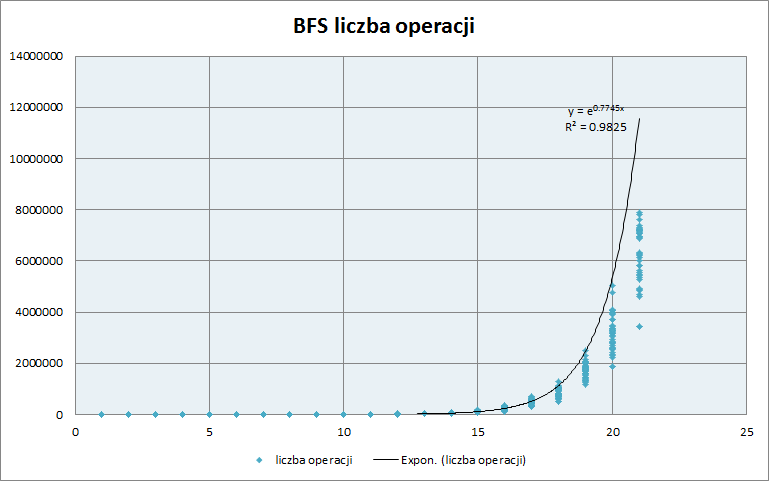
\includegraphics[scale=0.65]{pictures/BFS_operacje_exp.png}
	\caption{Breadth-First Search}
	\label{fig:Breadth-First Search}
\end{figure}

\begin{figure}[ht]
\centering
			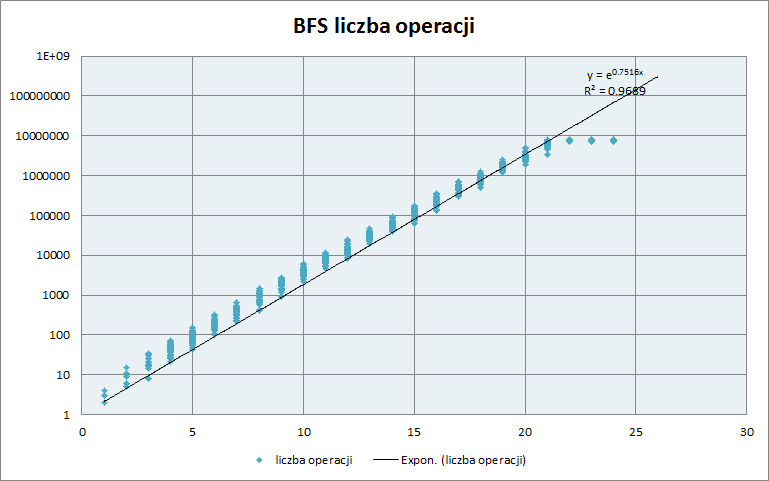
\includegraphics[scale=0.65]{pictures/BFS_operacje_log.png}
	\caption{Breadth-First Search}
	\label{fig:Breadth-First Search}
\end{figure}

\begin{figure}[ht]
\centering
			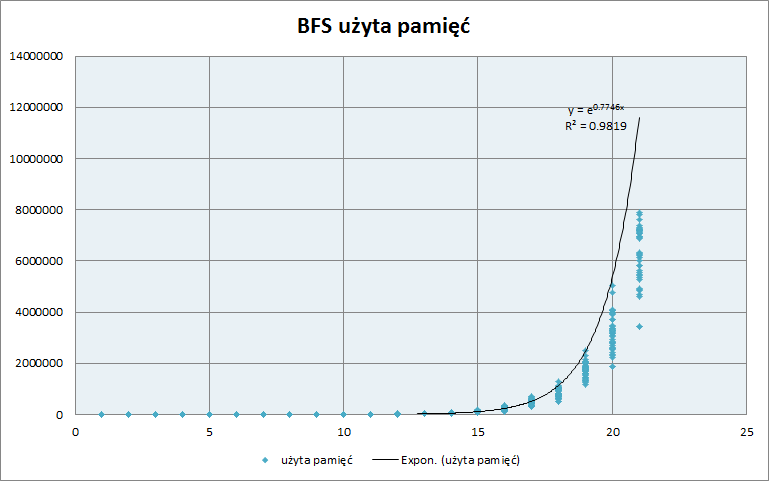
\includegraphics[scale=0.65]{pictures/BFS_pamiec_exp.png}
	\caption{Breadth-First Search}
	\label{fig:Breadth-First Search}
\end{figure}

\begin{figure}[ht]
\centering
			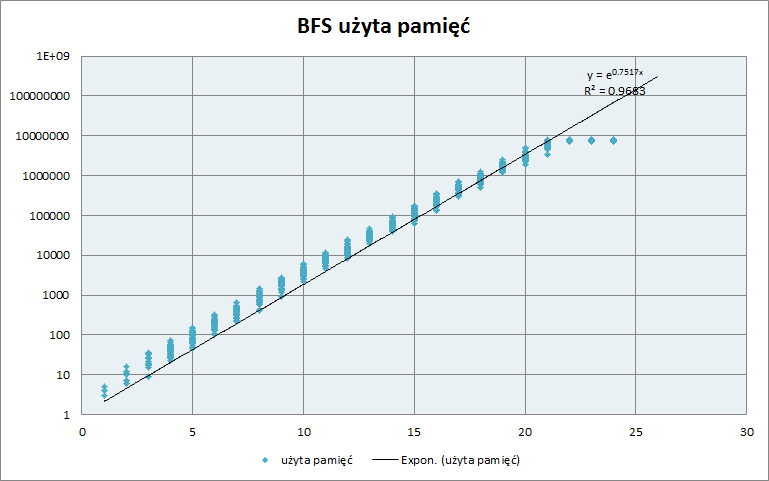
\includegraphics[scale=0.65]{pictures/BFS_pamiec_log.png}
	\caption{Breadth-First Search}
	\label{fig:Breadth-First Search}
\end{figure}

\begin{figure}[ht]
\centering
			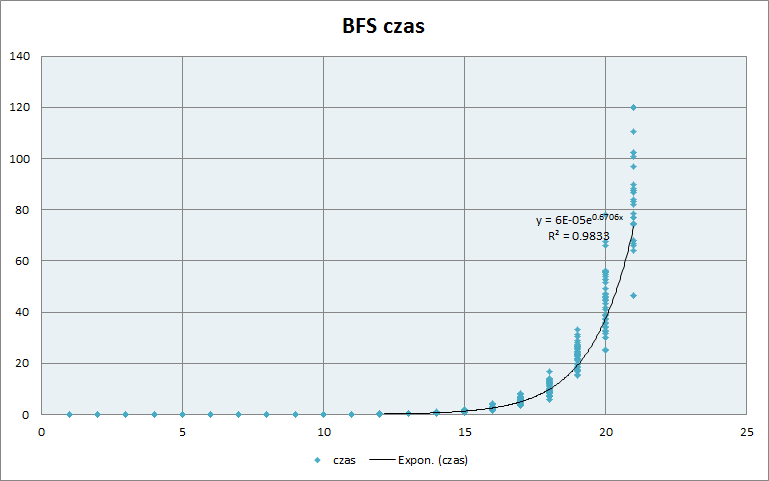
\includegraphics[scale=0.65]{pictures/BFS_czas_exp.png}
	\caption{Breadth-First Search}
	\label{fig:Breadth-First Search}
\end{figure}

\begin{figure}[ht]
\centering
			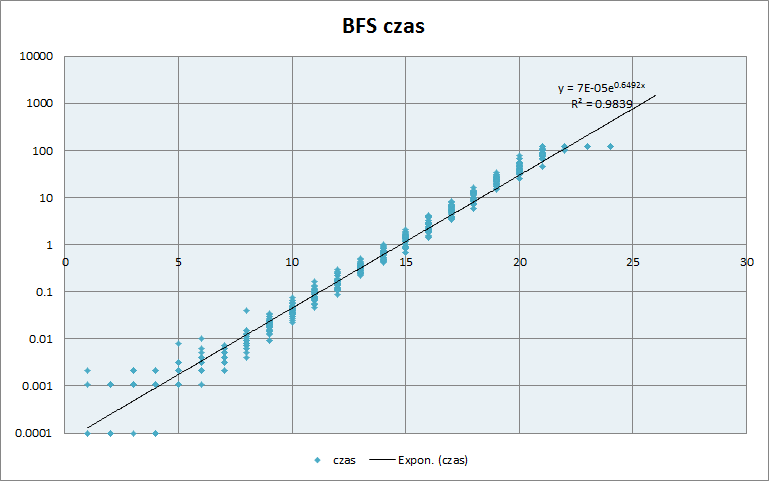
\includegraphics[scale=0.65]{pictures/BFS_czas_log.png}
	\caption{Breadth-First Search}
	\label{fig:Breadth-First Search}
\end{figure}

\begin{figure}[ht]
\centering
			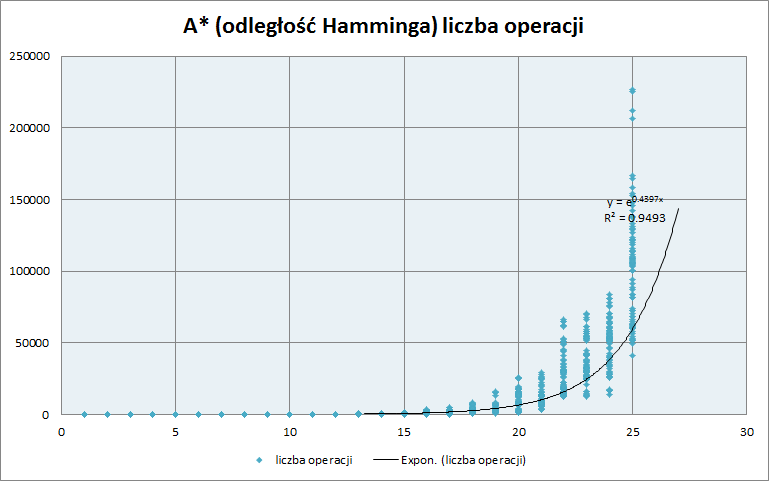
\includegraphics[scale=0.65]{pictures/A2_operacje_exp.png}
	\caption{A* Odleglosc Hamminga}
	\label{fig:A* Odleglosc Hamminga}
\end{figure}

\begin{figure}[ht]
\centering
			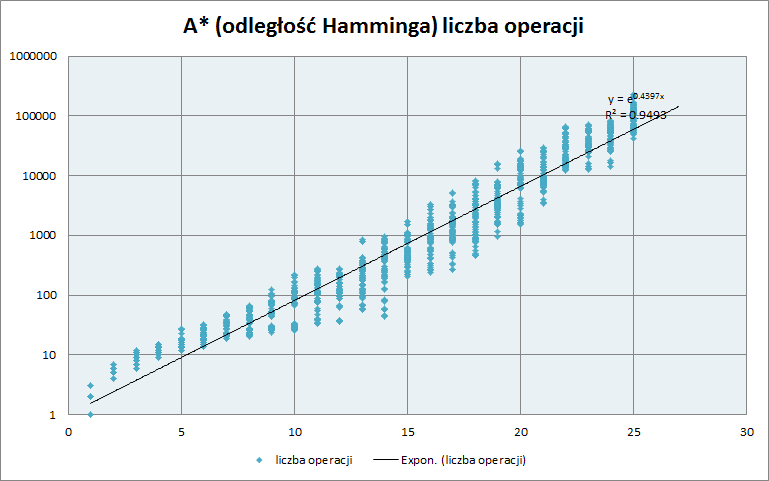
\includegraphics[scale=0.65]{pictures/A2_operacje_log.png}
	\caption{A* Odleglosc Hamminga}
	\label{fig:A* Odleglosc Hamminga}
\end{figure}

\begin{figure}[ht]
\centering
			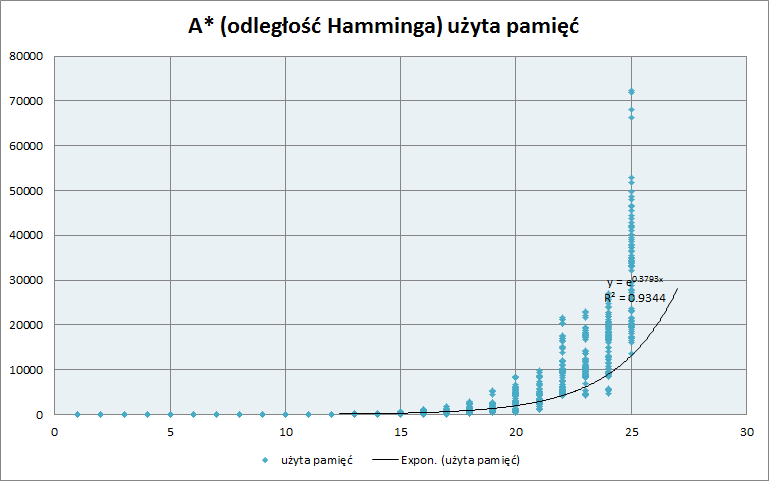
\includegraphics[scale=0.65]{pictures/A2_pamiec_exp.png}
	\caption{A* Odleglosc Hamminga}
	\label{fig:A* Odleglosc Hammingav}
\end{figure}

\begin{figure}[ht]
\centering
			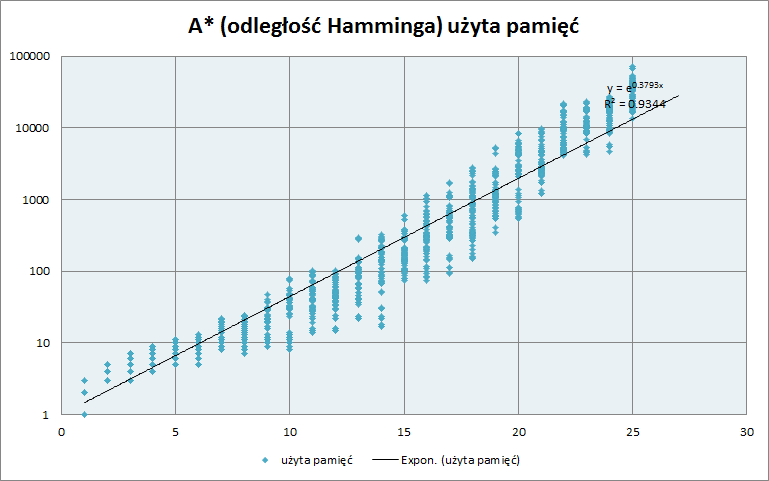
\includegraphics[scale=0.65]{pictures/A2_pamiec_log.png}
	\caption{A* Odleglosc Hamminga}
	\label{fig:A* Odleglosc Hamminga}
\end{figure}

\begin{figure}[ht]
\centering
			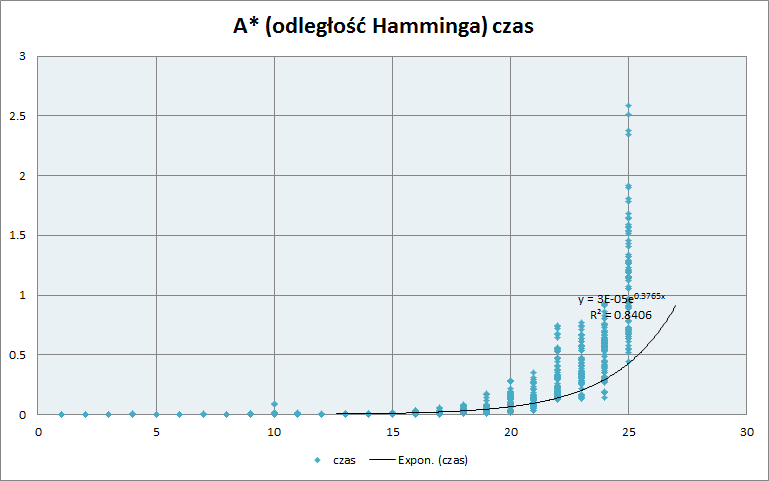
\includegraphics[scale=0.65]{pictures/A2_czas_exp.png}
	\caption{A* Odleglosc Hamminga}
	\label{fig:A* Odleglosc Hamminga}
\end{figure}

\begin{figure}[ht]
\centering
			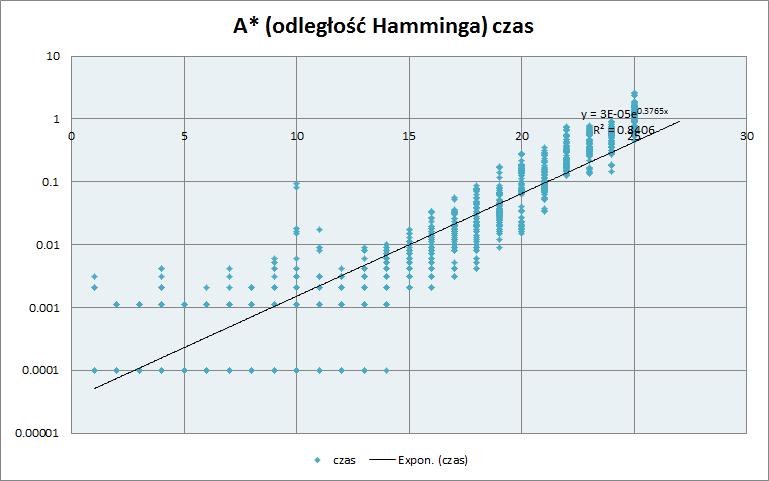
\includegraphics[scale=0.65]{pictures/A2_czas_log.png}
	\caption{A* Odleglosc Hamminga}
	\label{fig:A* Odleglosc Hamminga}
\end{figure}

\begin{figure}[ht]
\centering
			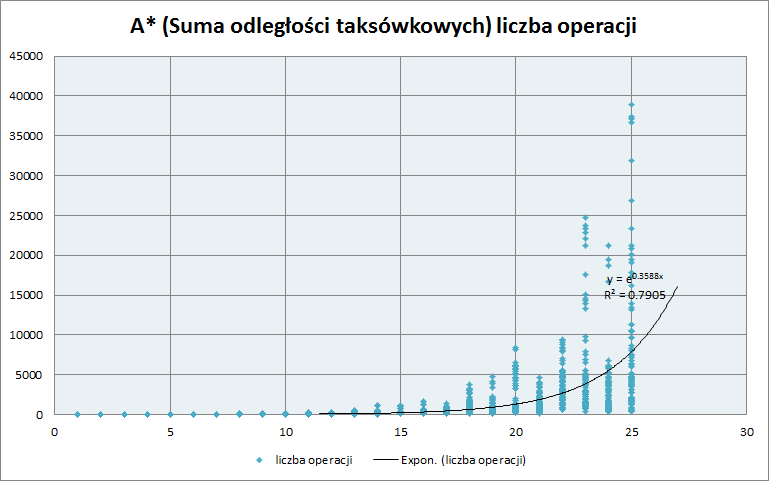
\includegraphics[scale=0.65]{pictures/A3_operacje_exp.png}
	\caption{A* Suma odleglosci taksowkowych}
	\label{fig:A* Suma odleglosci taksowkowych}
\end{figure}

\begin{figure}[ht]
\centering
			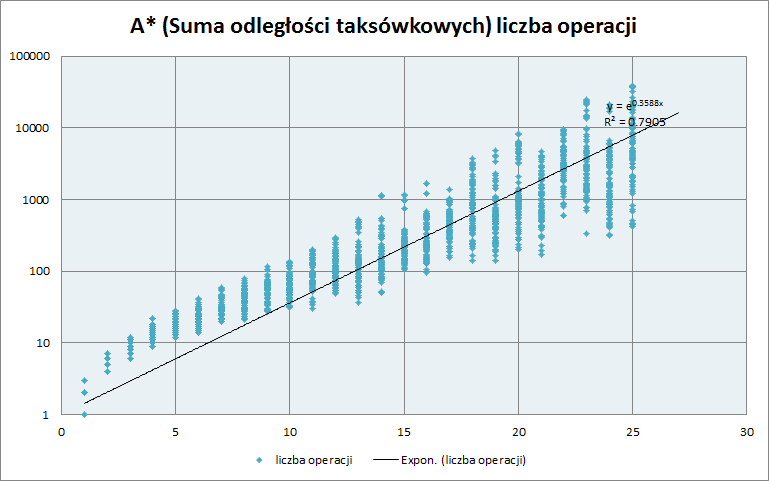
\includegraphics[scale=0.65]{pictures/A3_operacje_log.png}
	\caption{A* Suma odleglosci taksowkowych}
	\label{fig:A* Suma odleglosci taksowkowych}
\end{figure}

\begin{figure}[ht]
\centering
			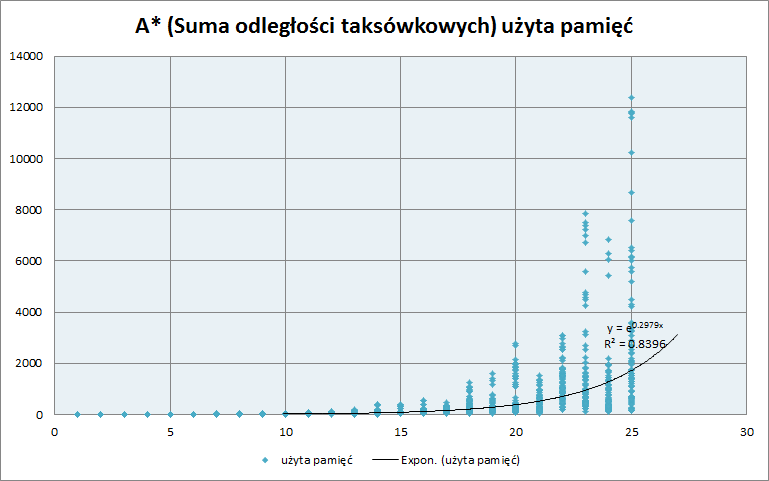
\includegraphics[scale=0.65]{pictures/A3_pamiec_exp.png}
	\caption{A* Suma odleglosci taksowkowych}
	\label{fig:A* Suma odleglosci taksowkowych}
\end{figure}

\begin{figure}[ht]
\centering
			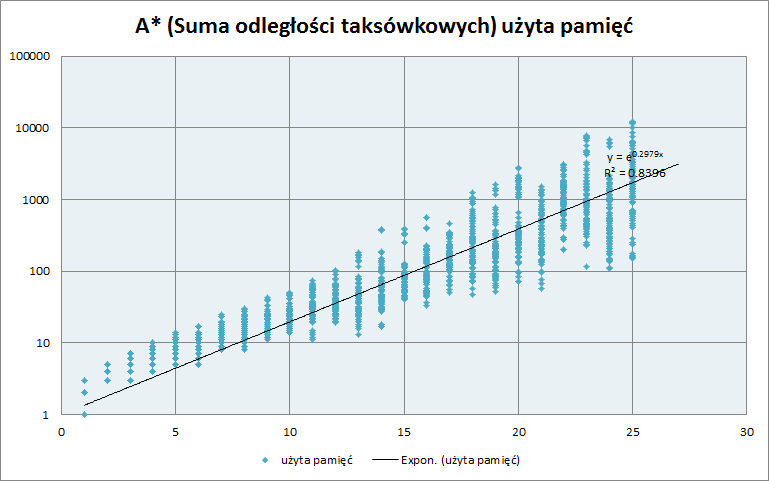
\includegraphics[scale=0.65]{pictures/A3_pamiec_log.png}
	\caption{A* Suma odleglosci taksowkowych}
	\label{fig:A* Suma odleglosci taksowkowych}
\end{figure}

\begin{figure}[ht]
\centering
			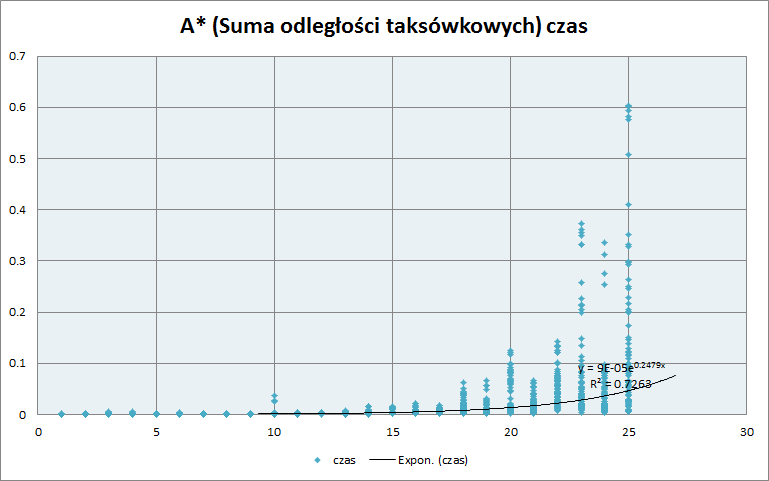
\includegraphics[scale=0.65]{pictures/A3_czas_exp.png}
	\caption{A* Suma odleglosci taksowkowych}
	\label{fig:A* Suma odleglosci taksowkowych}
\end{figure}

\begin{figure}[ht]
\centering
			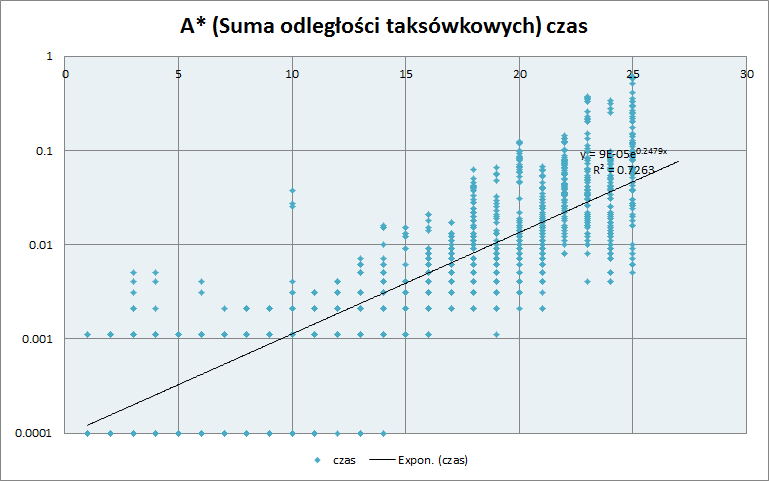
\includegraphics[scale=0.65]{pictures/A3_czas_log.png}
	\caption{A* Suma odleglosci taksowkowych}
	\label{fig:A* Suma odleglosci taksowkowych}
\end{figure}

\clearpage

\begin{figure}[ht]
\centering
			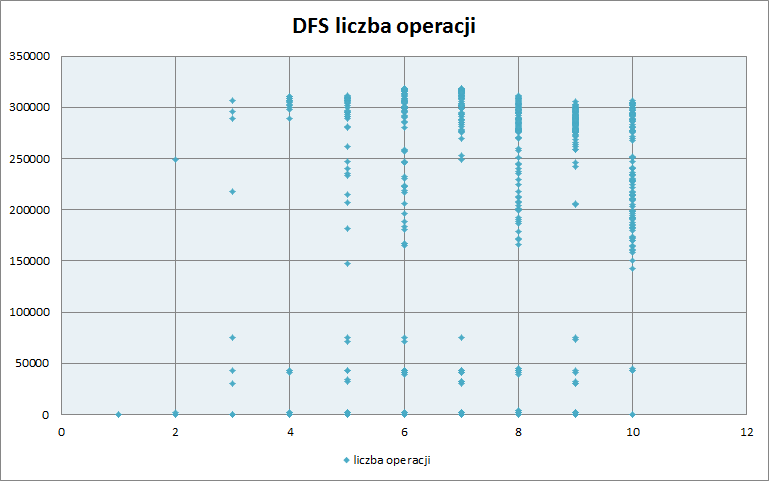
\includegraphics[scale=0.65]{pictures/DFS_operacje_exp.png}
	\caption{Depth-First Search}
	\label{fig:Depth-First Search}
\end{figure}

Po wyciągnięciu średniej z każdego przedziału otrzymujemy:

\begin{figure}[ht]
\centering
			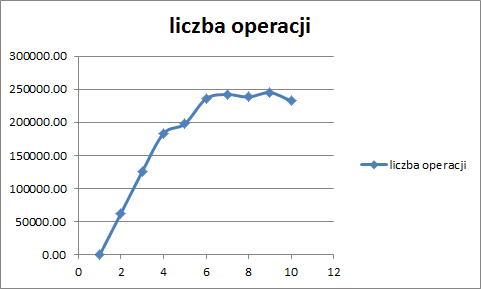
\includegraphics[scale=0.65]{pictures/old/dfs_operacje.png}
	\caption{Depth-First Search}
	\label{fig:Depth-First Search}
\end{figure}

\clearpage

\begin{figure}[ht]
\centering
			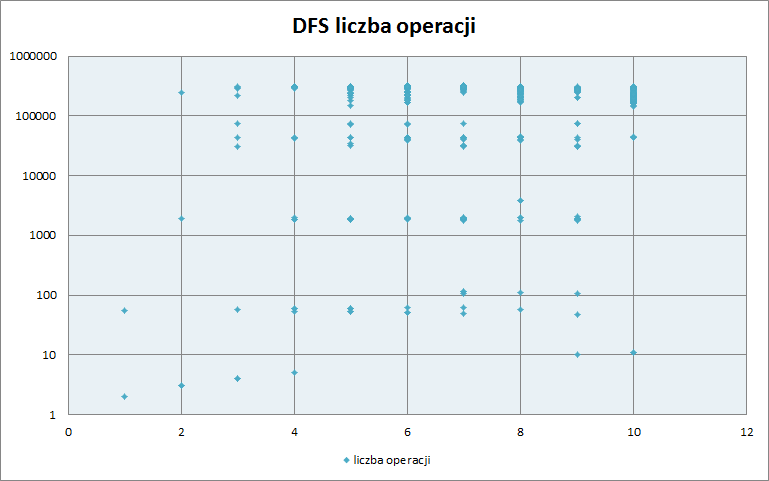
\includegraphics[scale=0.65]{pictures/DFS_operacje_log.png}
	\caption{Depth-First Search}
	\label{fig:Depth-First Search}
\end{figure}

\begin{figure}[ht]
\centering
			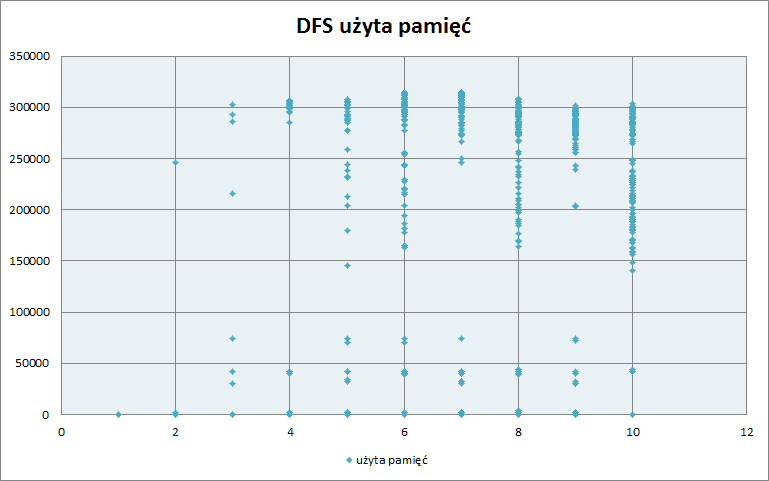
\includegraphics[scale=0.65]{pictures/DFS_pamiec_exp.png}
	\caption{Depth-First Search}
	\label{fig:Depth-First Search}
\end{figure}

\begin{figure}[ht]
\centering
			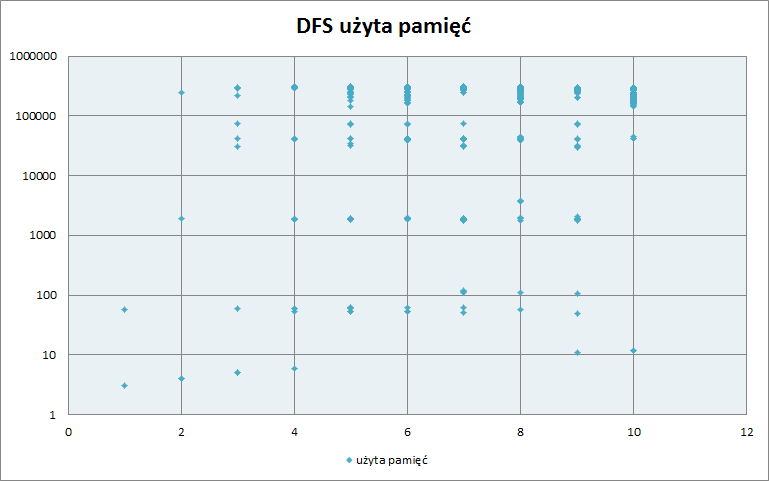
\includegraphics[scale=0.65]{pictures/DFS_pamiec_log.png}
	\caption{Depth-First Search}
	\label{fig:Depth-First Search}
\end{figure}

\begin{figure}[ht]
\centering
			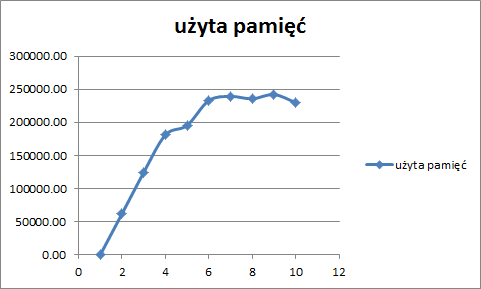
\includegraphics[scale=0.65]{pictures/old/dfs_space.png}
	\caption{Depth-First Search}
	\label{fig:Depth-First Search}
\end{figure}

\begin{figure}[ht]
\centering
			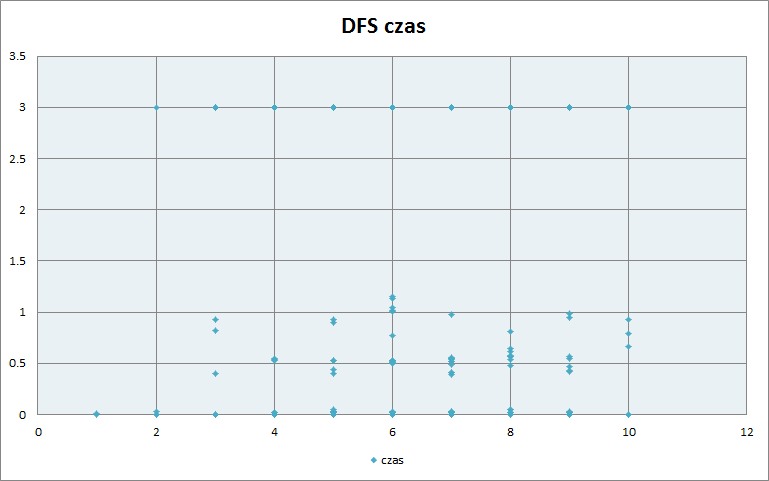
\includegraphics[scale=0.65]{pictures/DFS_czas_exp.png}
	\caption{Depth-First Search}
	\label{fig:Depth-First Search}
\end{figure}

\begin{figure}[ht]
\centering
			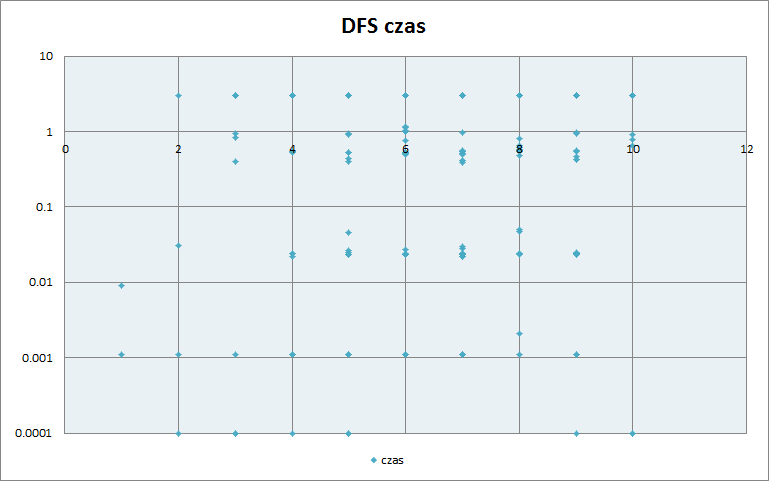
\includegraphics[scale=0.65]{pictures/DFS_czas_log.png}
	\caption{Depth-First Search}
	\label{fig:Depth-First Search}
\end{figure}

\begin{figure}[ht]
\centering
			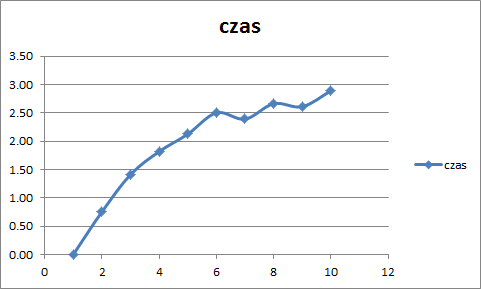
\includegraphics[scale=0.65]{pictures/old/dfs_time.png}
	\caption{Depth-First Search}
	\label{fig:Depth-First Search}
\end{figure}


\clearpage

\section{Wnioski}
  Najwydajniejszymi algorytmami okazały się, zgodnie z oczekiwaniami, algorytmy wykorzystujące heurystykę. Spowodowane jest to tym, że wybierane są tutaj drogi, które są najbliżej rozwiązania porzucając pozostałe. Funkcjonalności tej pozbawione są algorytmy nie wykorzystujące heurystyk, przez co rośnie czas poszukiwania. Najmniej wydajnym algorytmem okazał się DFS, ponieważ liczba iteracji jest tutaj największa.


	
	
	
\begin{thebibliography}{0}
  \bibitem{l2short} T. Oetiker, H. Partl, I. Hyna, E. Schlegl.
    \textsl{Nie za krótkie wprowadzenie do systemu \LaTeX2e}, 2007, dostępny
    online.
  \bibitem{klesk_grafy} Przemysław Klęsk.
    \textsl{Algorytmy przeszukiwania grafów i drzew dla gier i łamigłówek}, \url{http://wikizmsi.zut.edu.pl/uploads/b/be/2_search.pdf}
   \bibitem{wiki_bfs} Wikipedia, wolna encykolpedia
    \textsl{Breadth-first search}, \url{http://en.wikipedia.org/wiki/Breadth-first_search}
    \bibitem{wiki_astar} Wikipedia, wolna encyklopedia
    \textsl{Algorytm A*}, \url{http://pl.wikipedia.org/wiki/Algorytm_A*}
\end{thebibliography}
\end{document}